\chapter*{{\FontH{\Huge Flieg, Pinarella!}}\\\small \color{red} Grosi gewidmet}
\addcontentsline{toc}{chapter}{Flieg, Pinarella!}
\lettrine[lines=3]{\color{red}P}{inarella} war ein Schmetterling. Träge lag sie wie jeden Morgen auf dem Regal im Wohnzimmer der Familie Emil und liess sich die Sonne auf die Flügel scheinen. Sie gähnte, so laut das Schmetterlingsdamen eben können, und blickte sich gelangweilt im Zimmer um. Pinarella war nämlich kein einfacher Schmetterling, nein, sie bestand aus einem Körper aus Holz und die Flügel waren aus bunter Folie gemacht. Schön sah das zwar aus, aber zum Fliegen taugte so ein Körper nicht. Cornelia, die Tochter der Emils, hatte Pinarella gebastelt, als sie so ungefähr in der dritten Klasse gewesen war. Aber das war jetzt schon viele Jahre her, Cornelia hatte selbst schon zwei Kinder und mit denen war sie gerade zu Besuch bei ihren Eltern. 

Eigentlich wohnte Pinarella gar nicht auf dem Regal, sondern hing für gewöhnlich an einer Schnur über dem Ofen. Aber das letzte Mal, als Cornelia mit den Enkelinnen dagewesen war, war sie beim Spielen auf dem Boden gelandet und von da hat sie jemand auf das Regal gelegt. Bisher hatte sich noch niemand die Mühe gemacht, sie wieder aufzuhängen, aber das war Pinarella egal. Beide Orte waren genau gleich langweilig, so viel war klar. Deswegen war es auch ganz gleichgültig, wo sie gelagert wurde.

Es war natürlich nicht immer so langweilig bei den Emils. Vor allem wenn die Enkelinnen zu Besuch waren, war etwas los. Besonders Jette, die jüngste Tochter von Cornelia, spielte gerne mit dem Schmetterling. Jette war allerdings noch zu jung, um die Schönheit Pinarellas zu verstehen. Sonst würde sie wahrscheinlich nicht gar so garstig und nachlässig mit ihr umgehen. Mal wurde sie an den Flügeln gezogen, die dann umständlich von Frau Emil wieder festgeleimt werden mussten, dann wurde sie unachtsam unter einem Berg Legosteine vergraben. Und einmal wurde sie sogar mit auf die Pergola genommen und dann dort vergessen. Die ganze Nacht fror Pinarella ganz fürchtlerlich.

Jette war allerdings ein liebes Kind, das wusste Pinarella, deswegen nahm sie ihr das alles auch nicht übel. Sie war einfach noch zu jung. So viel wusste Pinarella über die Menschen: Wenn sie klein sind, überlegen sie manchmal nicht, was so alles passieren kann, wenn sie dies und jenes machen. Gerade gestern ist Jette alleine in ihr Stühlchen geklettert und dabei sehr unsanft abgestürzt. Das war ein Weinen! Und Jette hat sich selbst bestimmt nicht mit Absicht wehgetan, überlegte Pinarella, und deshalb war es wohl auch nicht böse gemeint, wenn Jette ihr mal wieder einen Fühler abgebissen hatte.

\afterpage{
\begin{figure}
    \thispagestyle{empty}
    \centering
    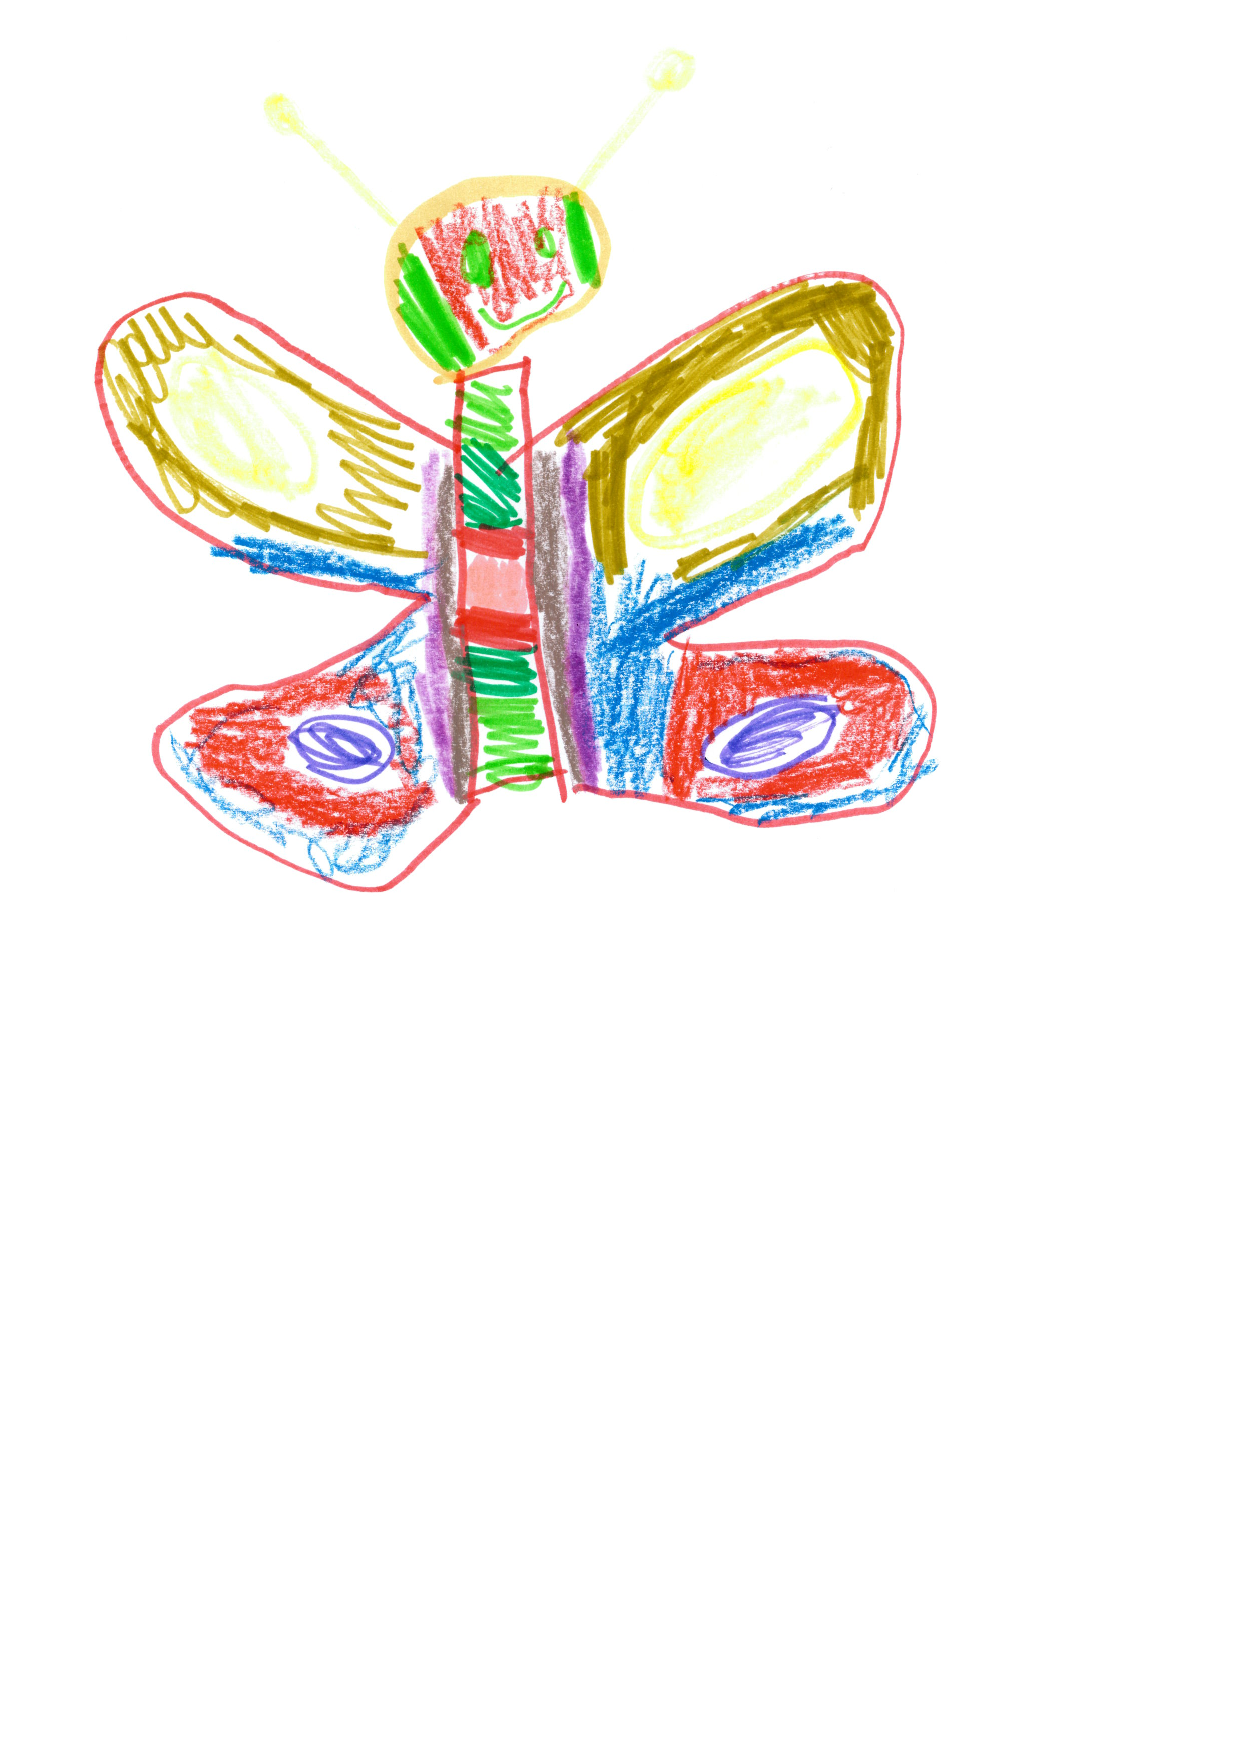
\includegraphics[width=\textwidth]{bilder/pinarella.pdf}
\end{figure}
\clearpage
}

An diesem Morgen war Jette wie so oft sehr früh munter geworden. Um den Papa nicht zu wecken, war Cornelia mit Jette ins Wohnzimmer gekommen. Da Jette auch in der Nacht schon mehrmals Lust gehabt hatte zu spielen, war ihre Mama noch sehr müde und wieder auf der Couch eingedöst. Jette spielte ein bisschen gelangweilt mit bunten Glasuntersetzern. 

Pinarella spienzelte vom Regal herab.  Auf dem Regal war sie jetzt zwar sicher vor Jette, aber eben auch alleine. Jette war viel zu klein, um so weit hoch zu kommen. Lieber wieder einen Flügel verlieren, dachte Pinarella, als den ganzen Tag hier zu liegen und nichts zu machen.

\enquote{Schade}, seufzte Pinarella, \enquote{wirklich schade, dass ich kein richtiger Schmetterling bin. Da wäre es ja doch viel lustiger, wenn ich ind die Welt hinaus fliegen könnte, um mit anderen Schmetterlingen zu spielen.} 

Jette blickte auf.

\enquote{Was ist denn mit dir los?}, fragte sie. Pinarella war verwirrt. Schon oft hatte sie versucht mit Menschen zu reden, aber so laut sie auch geschrien hatte, nie hat sie jemand gehört.

\enquote{Kannst Du mich verstehen?}, fragte sie daher ganz ungläubig. 

Jette nickte bloss. 

\enquote{Mir ist langweilig}, sagte Pinarella, \enquote{niemand spielt mit mir, meine Flügel sind schon voller Staub.}

\enquote{Dann komm doch hier zu mir geflogen!}, schlug Jette vor, die den Unterschied zwischen einem echten Schmetterling und einem gebastelten noch nicht so genau kannte. Und obwohl Jette das gar nicht so richtig interessierte, erklärte Pinarella ihr den Unterschied. Ihr war das nämlich wichtig. Jette verstand nicht alles, aber eines war klar: Pinarella wollte auch gerne fliegen können, um mit anderen Schmetterlingen zu spielen. Das verstand Jette sogar gut, sie spielte ja auch am liebsten mit anderen Kindern.

\enquote{Dann helfe ich Dir!}, beschloss Jette, hatte aber noch keine Ahnung, wie. Aber das ist normal bei kleinen Kindern. Die beschliessen immer Sachen, von denen sie noch nicht wissen, wie man das dann genau macht. Zuerst musste Pinarella mal von dem Regal herunter, das war offensichtlich. Das Regal war schon sehr hoch, sogar noch höher als Papa gross ist, schätzte Jette. Der konnte einen aber hoch nehmen, wenn man die Arme in die Luft streckt, Regale machen so etwas wohl aber nicht. Jette hatte bereits ein bisschen Lebenserfahrung. Und die sagte ihr auch, dass man etwas zu Hilfe nehmen musste.

Die beide sahen sich im Zimmer um, was denn diese Hilfe sein könnte. Jette hatte plötzlich eine Idee. Wenn sie mit dem Wasserhahn vom Waschbecken spielen wollte, schob sie sich immer das Schemelchen hin und stieg darauf. Für das Waschbecken war sie nämlich auch noch zu klein. Aber das Schemlechen war natürlich im Badezimmer und wenn man dort hin wollte, würde Mama bestimmt munter werden. Pinarella und jette mussten seufzen. Da bemerkte Jette den Stuhl. Sie schaute zu Pinarella, wieder zum Stuhl und versuchte abszuschätzen, ob man so zu ihr hinauf käme. So leise es einem kleinen Kind eben möglich ist, lief Jette zu dem Stuhl und schob ihn vorsichtig in Richtung Regal.

\enquote{Mach keinen Quatsch!} Mama war von dem Quietschen munter geworden, drehte sich aber zum Glück nochmals auf die Seite und schlief weiter. Jette und Pinarella hatten den Atem angehalten, den Jette mit einem lauten {\itshape Pffff.} jetzt wieder raus liess. Das war knapp. Wenn Mama gemerkt hätte, was Jette vor hatte, wäre sie bestimmt dagegen gewesen. Ganz leise kletterte Jette jetzt auf den Stuhl. Noch immer reichte sie nicht bis oben hin. Zum Glück lag da der Rückenkratzer vom Opa, den konnte sie nehmen und tatsächlich! Es klappte! Jette kam gerade so bis an das obere Ende des Regals. Sie erwischte Pinarella an einem Fühler und zog sie vom Regal herunter. 

Mit einem leisen {\itshape Plopp} landete Pinarella auf der Couch, aber zum Glück weit genug von Mama entfernt. Jette kletterte vom Stuhl herunter, was gar nicht so einfach war, nahm Pinarella, öffnete das Fenster und mit einem lauten 

\enquote{Jippie, flieg Pinarella!}, warf Jette den Holzschmetterling aus dem Fenster.

Natürlich konnte Pinarella nicht fliegen. Sie stürzte jäh ab und raste in Richtung Boden. 

\enquote{Da wird bestimmt noch mehr kaputt gehen, als nur ein Fühler.}, dachte Pinarella. Gerade in dem Moment ging die Sonne hinter den Bergen auf. Und mitten im Sturz traf Pinarella der allererste Sonnenstrahl des Tages. Sie konnte ihn auf ihren Flügeln spüren, zuckte instinktiv zusammen und da geschah es. Ihre Flügel bewegten sich! Erst langsam, dann immer schneller und noch bevor Pinarella auf dem Boden aufschlug, flog sie. Aus der Spielzeugpinarella war ein richtiger Schmetterling geworden. Höher und immer höher flog sie, fast so hoch wie das Haus und wieder runter zu dem Blumen auf der Wiese und einfach immer weiter. Jette jubelte vor Freude und Mama, die von ihrem Geschrei munter geworden war, fragte ganz verschlafen, was da los ist.

\enquote{Und nur wegen einem Schmetterling machst du so einen Lärm, dass du mich weckst?} Jette musste lächeln, Mama hatte gar nicht gemerkt, dass sie selbst den Schmetterling gebastelt hatte, der da geflogen war.\hfill {\color{red}\decofourleft}
